% !TeX program = xelatex
\documentclass[12pt,a4paper]{ctexart}
\usepackage{geometry}
\geometry{left=2.5cm,right=2.5cm,top=2.5cm,bottom=2.5cm}
\usepackage{fancyhdr}
\usepackage{graphicx}
\usepackage{amsmath}
\usepackage{float}
\usepackage{caption}
\captionsetup{font=small,labelfont=bf}
\usepackage[hidelinks]{hyperref}
\usepackage{listings}
\usepackage{xcolor}
\usepackage{booktabs}
\usepackage{url}

\setlength{\headheight}{13.6pt}

\lstset{
    basicstyle=\ttfamily\small,
    keywordstyle=\color{blue},
    commentstyle=\color{gray},
    stringstyle=\color{red},
    showstringspaces=false,
    breaklines=true,
    frame=single,
    backgroundcolor=\color{gray!10},
    numbers=left,
    numberstyle=\tiny\color{gray},
    tabsize=4,
    xleftmargin=2em,
    xrightmargin=2em,
}

\setCJKmainfont{Noto Serif CJK SC}
\setCJKsansfont{Noto Sans CJK SC}
\setCJKmonofont{Noto Sans Mono CJK SC}

\pagestyle{fancy}
\fancyhf{}
\fancyhead[C]{\small 系统开发工具基础 · 实验报告（第四周）}
\fancyfoot[C]{\thepage}
\renewcommand{\headrulewidth}{0.4pt}
\renewcommand{\footrulewidth}{0pt}

\usepackage{titlesec}
\titleformat{\section}{\Large\bfseries\centering}{第\thesection 题}{1em}{}
\titleformat{\subsection}{\normalsize\bfseries}{\arabic{subsection}}{1em}{}
\renewcommand{\baselinestretch}{1.3}

\begin{document}

% ==================== 封面 ====================
\begin{center}
    {\Huge\bfseries 系统开发工具基础} \\[0.5cm]
    {\LARGE 每周课上实验报告} \\[0.8cm]
    {\large 第四周（2026年9月14日）} \\[2cm]
    \large
    \begin{tabular}{rl}
        姓\qquad 名： & 李永铖 \\[0.3cm]
        学\qquad 号： & 25030021039 \\[0.3cm]
        实验日期：    & 2026年9月14日 \\
    \end{tabular} \\[2cm]
    \today
\end{center}
\newpage

% ==================== 实验概况 ====================
\section*{实验概况}
\addcontentsline{toc}{section}{实验概况}

本次实验为第四周的四道课上练习题，涵盖代码质量（ruff、pytest、check.sh 质量门禁）、元编程与构建系统（Makefile 依赖重建）、大杂烩（本地 HTTP 服务 + curl + jq + Markdown 报告）以及课堂综合测试（修复并交付小型工具仓库）。通过动手实践，掌握了本地质量门禁的搭建流程、Make 依赖图的编写、jq 处理 JSON 数据的方法，以及基于 Git 的完整交付闭环。

\subsection*{实验环境}
\begin{itemize}
    \item 操作系统：Windows 11 + WSL2 (Debian trixie)
    \item Shell：bash 5.0
    \item Python 版本：3.13.5
    \item 已安装工具：Git、python3、pip、pytest、ruff、build、jq、shellcheck、bsdextrautils、pre-commit、coverage
    \item 包管理器：apt、pip
\end{itemize}

\subsection*{遇到的主要问题与解决}
\begin{enumerate}
    \item \textbf{复制 q10 为 q13 时出现目录嵌套}：第一次执行 \texttt{cp -r q10 q13} 前 q13 已存在，导致文件被放到 \texttt{q13/q10} 中。解决：先 \texttt{rm -rf q13} 再复制；若目标目录不存在，\texttt{cp -r} 会把源目录重命名为目标目录。
    \item \textbf{pip install -e . 构建出 UNKNOWN 空包}：因为在上一步错误的目录下执行，\texttt{pyproject.toml} 未包含在项目根。解决：确保 \texttt{pyproject.toml}、\texttt{src/}、\texttt{tests/} 在同一层再执行 \texttt{pip install -e .}。
    \item \textbf{python -m greetlab.cli 无任何输出}：\texttt{cli.py} 缺少 \texttt{if \_\_name\_\_ == "\_\_main\_\_": main()} 入口。解决：在文件末尾补上该入口。
    \item \textbf{ruff 报 PLW1510：subprocess.run 缺少 check 参数}：解决：显式加 \texttt{check=False}。
    \item \textbf{q16 从 q13 复制过来的 .venv 路径错乱}：虚拟环境内硬编码路径仍指向 q13，\texttt{sys.executable} 解析错误。解决：删除并重建虚拟环境。
    \item \textbf{jq 未安装}：\texttt{./api\_report.sh} 报 \texttt{jq: command not found}。解决：\texttt{sudo apt install -y jq}。
    \item \textbf{column 命令缺失}：\texttt{column: command not found}。解决：\texttt{sudo apt install -y bsdextrautils}。
    \item \textbf{make build 报 No module named build}：未激活虚拟环境，系统 Python 未安装 build。解决：\texttt{source .venv/bin/activate} 后 \texttt{pip install build}。
\end{enumerate}

\newpage

% ==================== 第13题 ====================
\section{建立可执行的本地质量门禁}

\subsection{任务目标}
复用第 10 题完成的 greetlab 包，在 q13 中建立一个轻量本地质量检查：为 ruff 和 pytest 配置最小配置，补充正常姓名和空白姓名两个测试，编写 \texttt{check.sh} 串联格式化、静态检查和测试，并保证脚本返回 0。

\subsection{操作步骤}
\begin{enumerate}
    \item 从 q10 复制项目为 q13，清理旧的 \texttt{.venv}、\texttt{dist}、\texttt{build} 和 \texttt{*.egg-info}。
    \item 在 \texttt{pyproject.toml} 中追加 \texttt{[tool.ruff]} 和 \texttt{[tool.pytest.ini\_options]} 配置。
    \item 编写 \texttt{tests/test\_cli.py}，包含 \texttt{test\_normal\_name} 与 \texttt{test\_blank\_name}。
    \item 创建虚拟环境并 \texttt{pip install -e .}、\texttt{pip install pytest ruff}。
    \item 依次运行 \texttt{ruff format .}、\texttt{ruff check . --fix}、\texttt{pytest}，修复问题。
    \item 编写 \texttt{check.sh}，串联 \texttt{ruff format --check}、\texttt{ruff check}、\texttt{pytest}。
\end{enumerate}

\subsection{关键代码}

\texttt{pyproject.toml} 追加内容：
\begin{lstlisting}
[tool.ruff]
line-length = 88
target-version = "py313"

[tool.pytest.ini_options]
minversion = "7.0"
testpaths = ["tests"]
python_files = "test_*.py"
python_classes = "Test*"
python_functions = "test_*"
\end{lstlisting}

\texttt{check.sh}：
\begin{lstlisting}[language=bash]
#!/usr/bin/env bash
set -e
echo "Running ruff format check..."
ruff format --check .
echo "Running ruff check..."
ruff check .
echo "Running pytest..."
pytest
echo "All checks passed!"
\end{lstlisting}

\subsection{运行结果}
\begin{lstlisting}
Running ruff format check...
4 files already formatted
Running ruff check...
All checks passed!
Running pytest...
collected 2 items
tests/test_cli.py ..                                     [100%]
====================== 2 passed in 0.10s ======================
All checks passed!
\end{lstlisting}

\subsection{演示截图}
\begin{figure}[H]
    \centering
    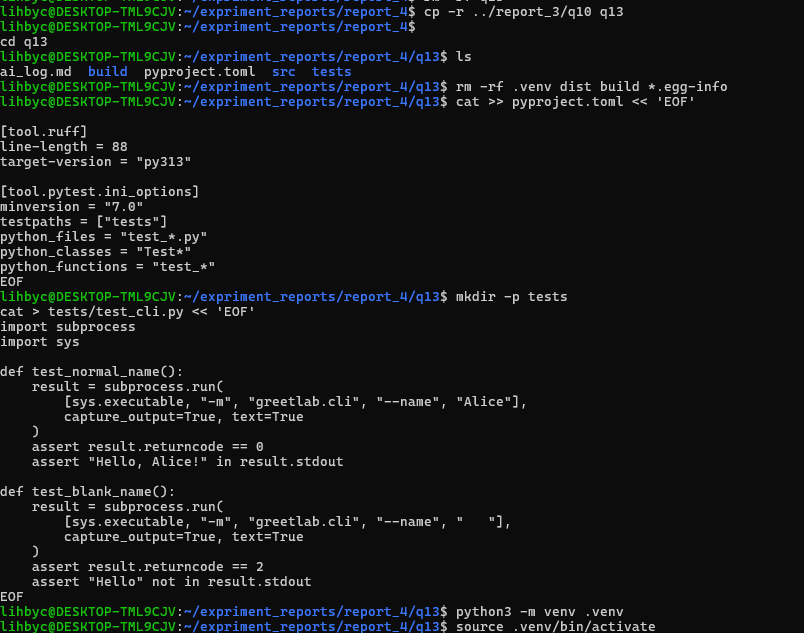
\includegraphics[width=0.85\textwidth]{q011.png}
    \caption{check.sh 全部通过}
    \label{fig:q13_check}
\end{figure}
\par
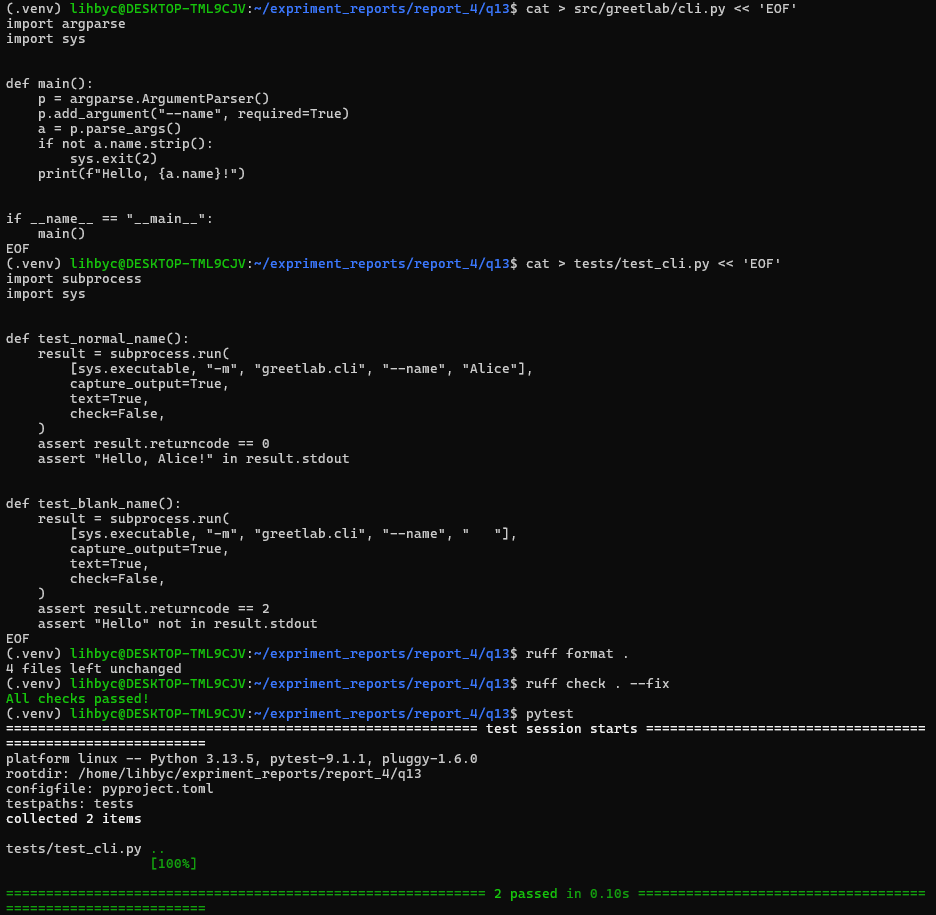
\includegraphics[width=0.85\textwidth]{q012.png}
\par
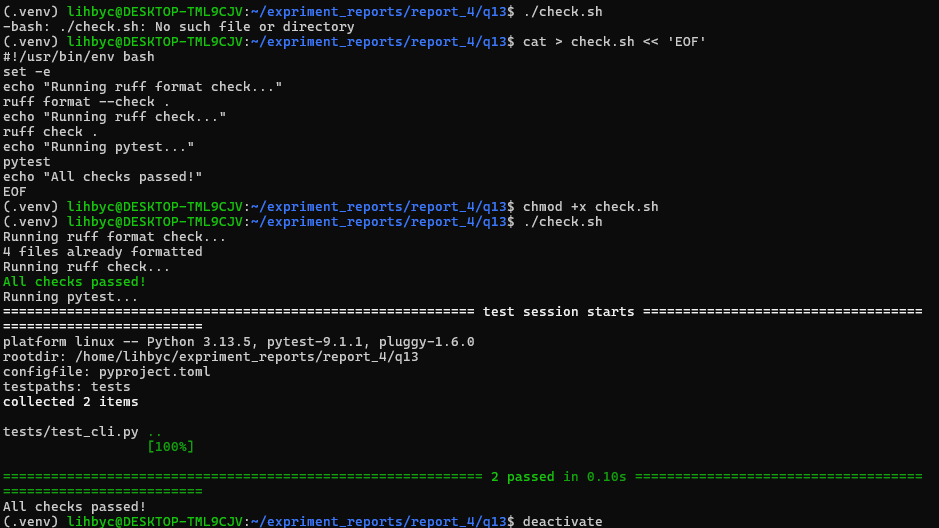
\includegraphics[width=0.85\textwidth]{q013.png}
\newpage

% ==================== 第14题 ====================
\section{让 Make 只重建真正受影响的产物}

\subsection{任务目标}
在 q14 中创建 \texttt{data.csv}、\texttt{stats.py}、\texttt{build\_report.py} 和 \texttt{report.md}，编写 Makefile，包含 \texttt{all}、\texttt{stats.txt}、\texttt{report.txt} 和 \texttt{clean} 目标，验证依赖驱动的增量构建。

\subsection{操作步骤}
\begin{enumerate}
    \item 用 heredoc 创建四个源文件。
    \item 编写 Makefile，准确声明数据文件、脚本与中间产物的依赖。
    \item 首次 \texttt{make}，生成 \texttt{stats.txt} 与 \texttt{report.txt}。
    \item 再次 \texttt{make}，验证无改动时不执行配方。
    \item \texttt{touch data.csv} 后 \texttt{make}，确认两个产物重新生成。
    \item \texttt{make clean}，只删除生成物，保留源文件。
\end{enumerate}

\subsection{关键代码}

Makefile：
\begin{lstlisting}
.PHONY: all clean

all: report.txt

stats.txt: data.csv stats.py
	python3 stats.py

report.txt: report.md stats.txt build_report.py
	python3 build_report.py

clean:
	rm -f stats.txt report.txt
\end{lstlisting}

\subsection{运行结果}
\begin{lstlisting}
$ make
python3 stats.py
python3 build_report.py

$ make
make: Nothing to be done for 'all'.

$ touch data.csv
$ make
python3 stats.py
python3 build_report.py

$ make clean
rm -f stats.txt report.txt
\end{lstlisting}

\subsection{演示截图}
\begin{figure}[H]
    \centering
    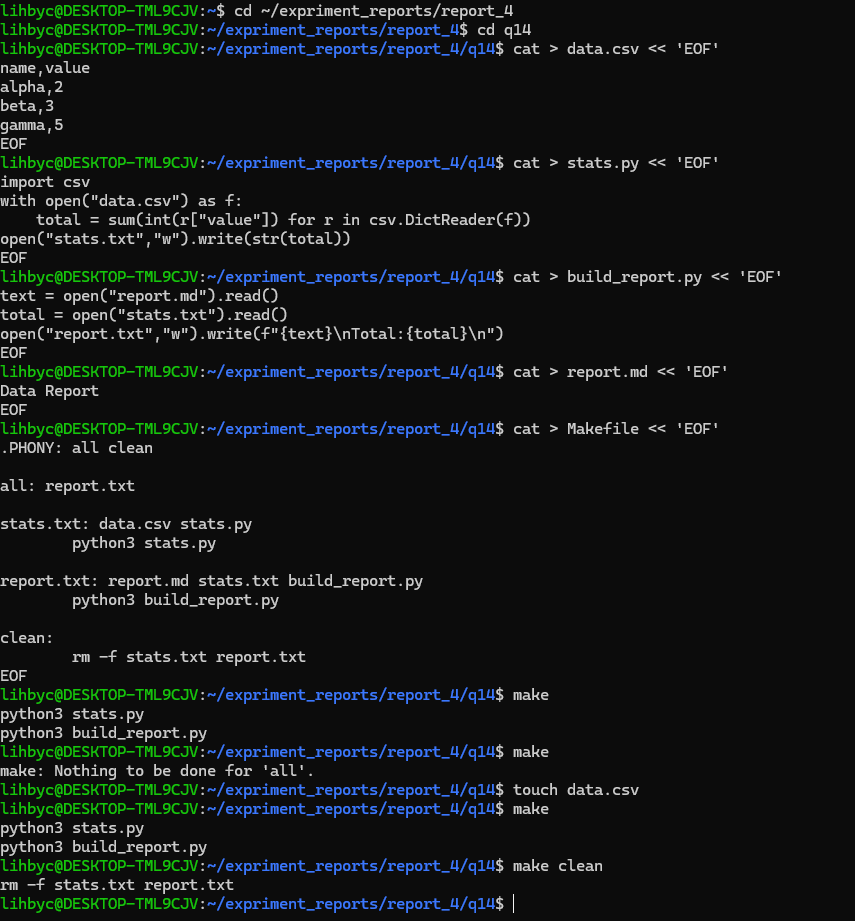
\includegraphics[width=0.85\textwidth]{q021.png}
    \caption{Make 增量构建验证}
    \label{fig:q14_make}
\end{figure}

\newpage

% ==================== 第15题 ====================
\section{把本地 API 数据转换为可读报告}

\subsection{任务目标}
在 q15 中创建给定 JSON 并启动本地 HTTP 服务，用 \texttt{curl} 与 \texttt{jq} 生成简短 Markdown 报告。

\subsection{操作步骤}
\begin{enumerate}
    \item 将给定 JSON 保存为 \texttt{packages.json}。
    \item 在 q15 目录运行 \texttt{python3 -m http.server 8000} 并置于后台。
    \item 编写 \texttt{api\_report.sh}：\texttt{curl -fsS} 获取数据，\texttt{jq} 筛选 \texttt{status=="active" and downloads>=100}，按 \texttt{downloads} 降序、\texttt{name} 升序排列，生成 \texttt{summary.json}，再转换为 \texttt{summary.md}。
    \item 运行脚本并查看 \texttt{summary.md}。
\end{enumerate}

\subsection{关键代码}

\texttt{api\_report.sh}：
\begin{lstlisting}[language=bash]
#!/usr/bin/env bash
set -e
URL="http://127.0.0.1:8000/packages.json"

curl -fsS "$URL" | jq '
  map(select(.status == "active" and .downloads >= 100))
  | sort_by(-.downloads, .name)
  | { title: "Active Packages Report",
      table: [.[] | {name, version, downloads}] }
' > summary.json

jq -r '
  "## " + .title + "\n",
  "| Name | Version | Downloads |",
  "|------|---------|-----------|",
  (.table[] | "| " + .name + " | " + .version + " | " + (.downloads|tostring) + " |")
' summary.json > summary.md

rm summary.json
\end{lstlisting}

\subsection{运行结果}
\begin{lstlisting}
$ cat summary.md
## Active Packages Report

| Name | Version | Downloads |
|------|---------|-----------|
| delta | 0.9.0 | 450 |
| gamma | 1.5.1 | 450 |
| alpha | 1.2.0 | 120 |
\end{lstlisting}

\subsection{演示截图}
\begin{figure}[H]
    \centering
    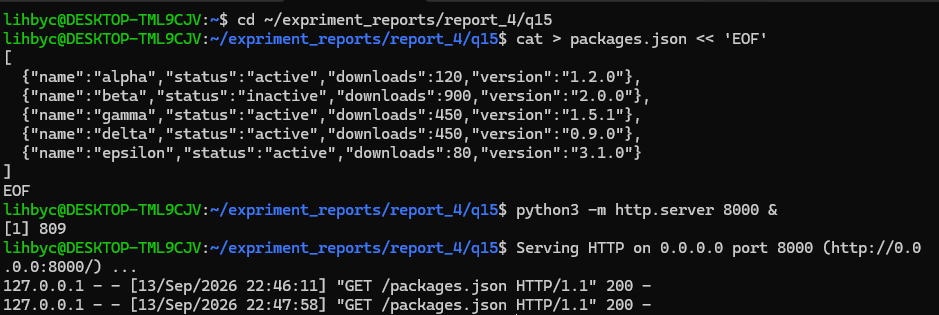
\includegraphics[width=0.85\textwidth]{q031.png}
    \caption{HTTP 服务与 summary.md 生成}
    \label{fig:q15_report}
\end{figure}
\par
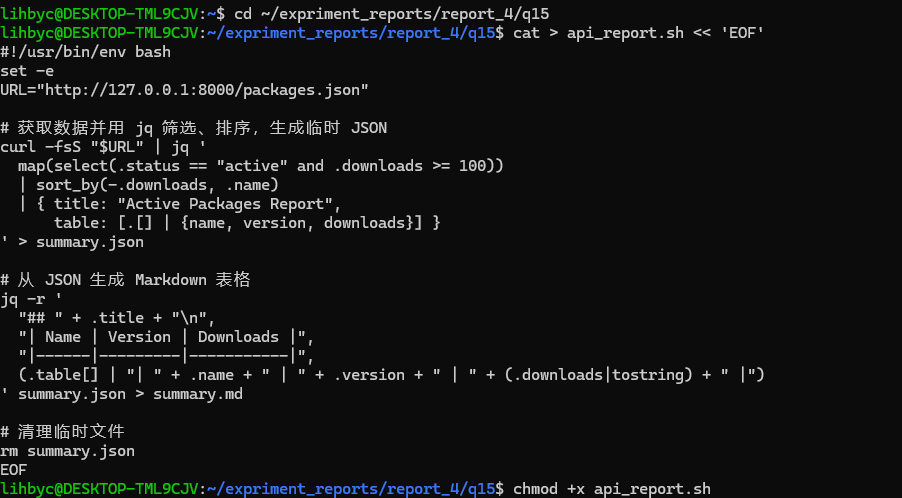
\includegraphics[width=0.85\textwidth]{q032.png}
\par
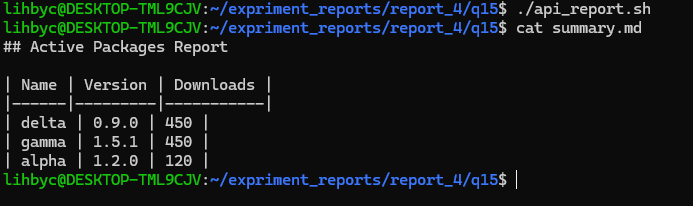
\includegraphics[width=0.85\textwidth]{q033.png}
\newpage

% ==================== 第16题 ====================
\section{修复并交付一个陌生的小型工具仓库}

\subsection{任务目标}
复用第 13 题的项目，在 q16 中完成一次综合检查：故意破坏问候语实现、确认测试失败、修复、编写最小 Makefile（check/build/clean）、构建 wheel、计算 SHA-256，并以内容聚焦的 Git 提交收尾。

\subsection{操作步骤}
\begin{enumerate}
    \item 从 q13 复制为 q16，初始化 Git 仓库并完成初始提交。
    \item 用 \texttt{sed} 把 \texttt{print(f"Hello, \{a.name}!")} 改为 \texttt{print("Hello, name!")}，运行 \texttt{./check.sh} 确认测试失败。
    \item 修复 \texttt{cli.py}，恢复正确输出并保留空白校验；补上 \texttt{\_\_main\_\_} 入口。
    \item 编写 Makefile，包含 \texttt{check}、\texttt{build}、\texttt{clean}。
    \item 重建虚拟环境，安装 \texttt{pytest}、\texttt{ruff}、\texttt{build}，运行 \texttt{make check} 与 \texttt{make build}。
    \item \texttt{sha256sum dist/*.whl} 计算 wheel 哈希。
    \item \texttt{git add .} 并提交一个内容聚焦的 commit。
\end{enumerate}

\subsection{关键代码}

Makefile：
\begin{lstlisting}
.PHONY: check build clean

check:
	./check.sh

build:
	python3 -m build --wheel

clean:
	rm -rf dist/ build/ *.egg-info
\end{lstlisting}

\subsection{运行结果}
\begin{lstlisting}
$ make build
Successfully built greetlab_25030021039-0.1.0-py3-none-any.whl

$ sha256sum dist/*.whl
5a6af2d8ed1887de39bdb9600c981ed31a3f0c7961a87049615d7d78f3286475
  dist/greetlab_25030021039-0.1.0-py3-none-any.whl

$ git log --oneline
55ae357 (HEAD -> master) fix: restore correct greeting and add Makefile for check/build/clean
b9e72f2 Initial commit: copy from q13 with quality gate
\end{lstlisting}

\subsection{演示截图}
\begin{figure}[H]
    \centering
    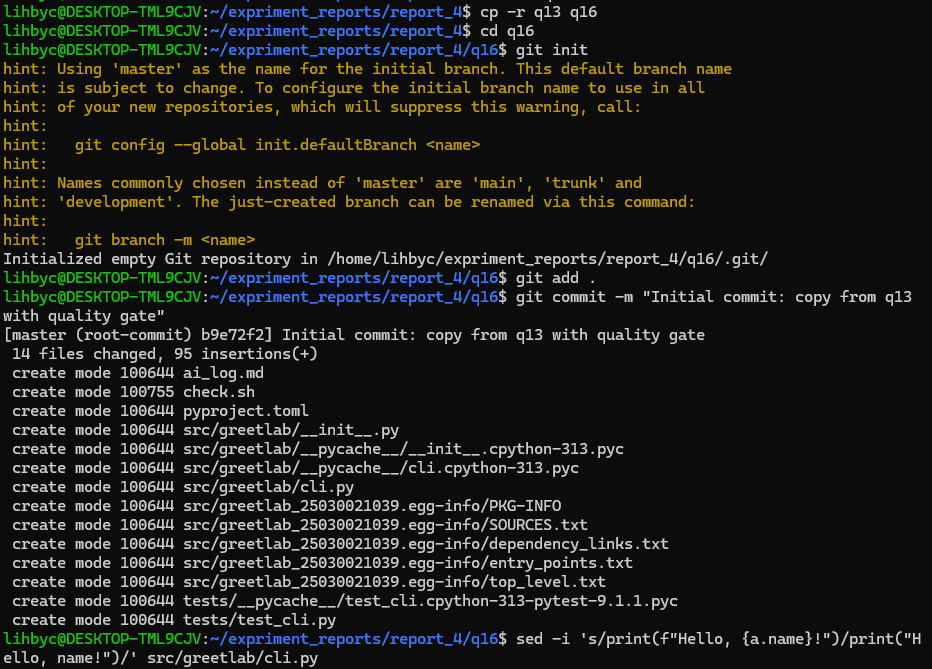
\includegraphics[width=0.85\textwidth]{q041.png}
    \caption{make build 与 SHA-256}
    \label{fig:q16_build}
\end{figure}
\par
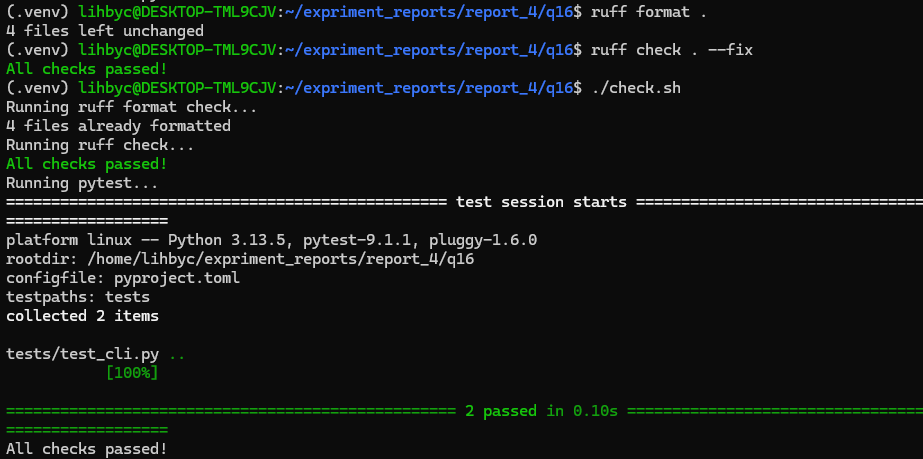
\includegraphics[width=0.85\textwidth]{q042.png}
\par
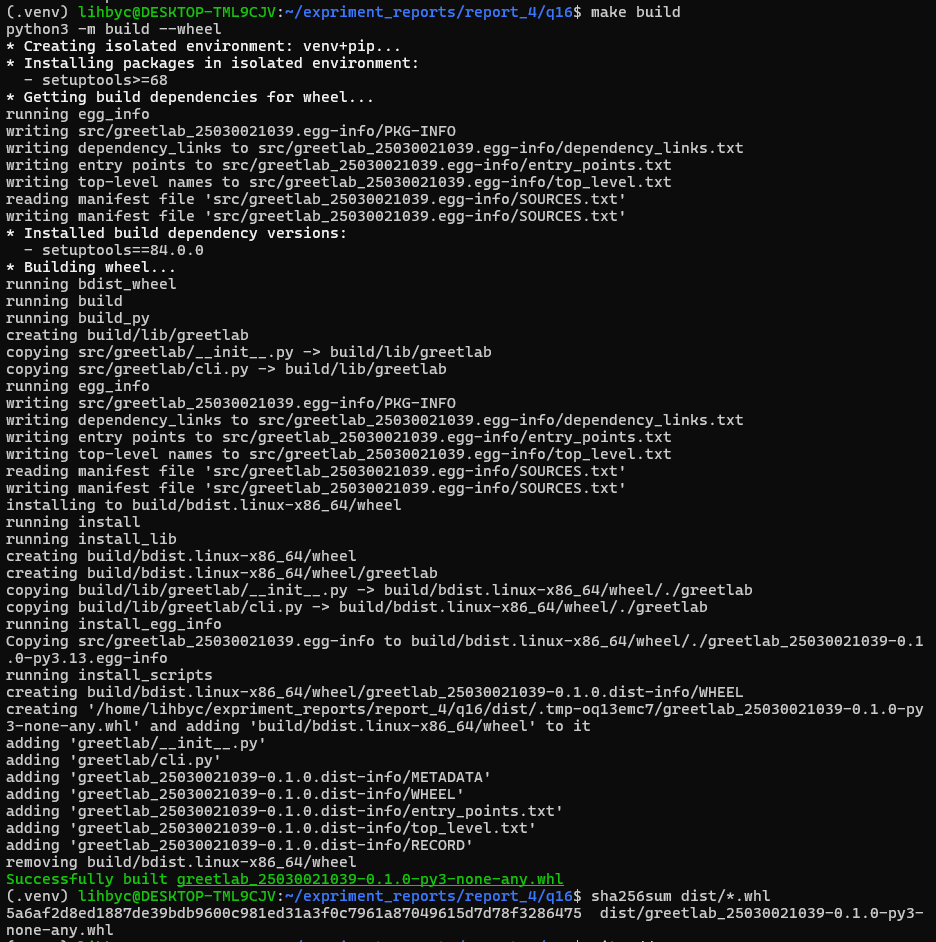
\includegraphics[width=0.85\textwidth]{q043.png}
\par
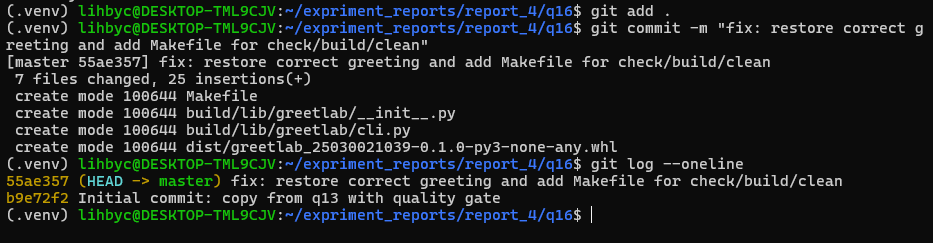
\includegraphics[width=0.85\textwidth]{q044.png}
\begin{figure}[H]
    \centering
    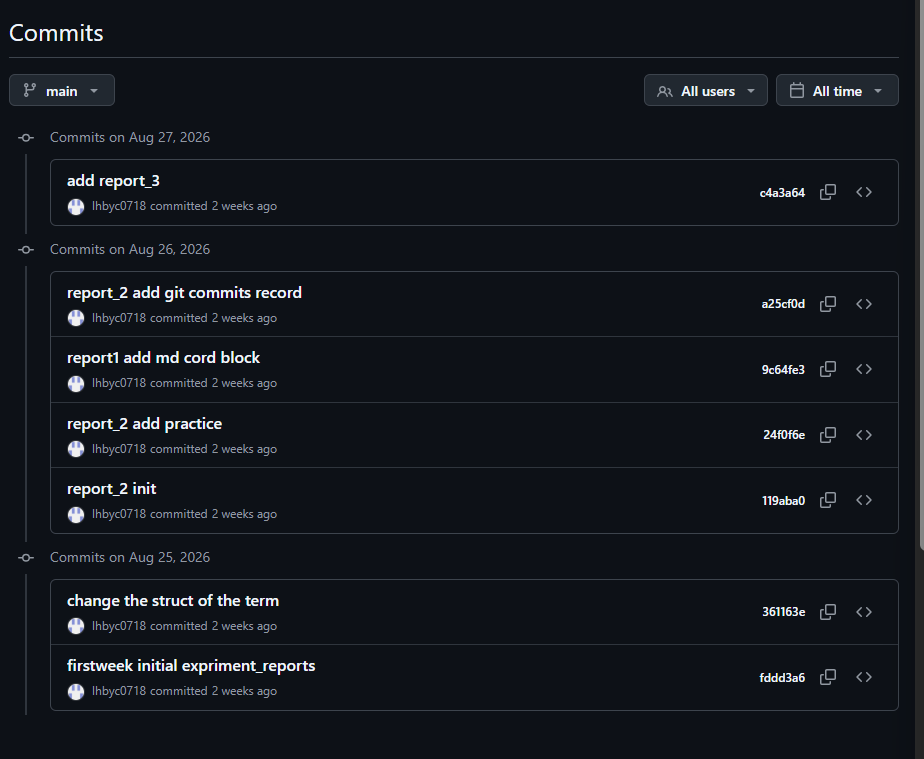
\includegraphics[width=0.85\textwidth]{git_commits_week4.png}
    \caption{Git 提交记录}
    \label{fig:q16_git}
\end{figure}

\newpage

% ==================== 课后练习 ====================
\section*{课后练习}
\addcontentsline{toc}{section}{课后练习}

以下为本周的 12 项课后拓展练习，涵盖代码质量、正则表达式、元编程与构建、JSON 解析与命令行工具等方向。所有练习均在本地 WSL2 (Debian) 环境中完成，目录为 \texttt{report\_4/practice/p01} 至 \texttt{p12}，操作日志完整可复现。

% ---------- p01 ----------
\subsection*{练习1（p01）：用 ruff 格式化并检查代码}
\textbf{内容}：体会自动格式化与 linter 检查的差别。

\textbf{操作步骤}：
\begin{enumerate}
    \item \texttt{cat > messy.py} 写入含未使用导入、多余空格的代码。
    \item \texttt{ruff format messy.py} 只改格式。
    \item \texttt{ruff check messy.py} 报出 I001、F401 等问题。
    \item \texttt{ruff check messy.py --fix} 自动修复未使用导入并整理导入顺序。
\end{enumerate}

\textbf{结果}：
\begin{lstlisting}
$ ruff check messy.py
Found 3 errors.
[*] 3 fixable with the `--fix` option.

$ ruff check messy.py --fix
Found 2 errors (2 fixed, 0 remaining).
\end{lstlisting}
\par

\includegraphics[width=0.85\textwidth]{p011.png}
\par

\includegraphics[width=0.85\textwidth]{p012.png}
\textbf{解题感悟}：ruff format 与 ruff check 各司其职，前者管格式，后者管语义；\texttt{--fix} 能自动处理大部分机械问题。

\vspace{0.3cm}

% ---------- p02 ----------
\subsection*{练习2（p02）：配置 pre-commit 钩子}
\textbf{内容}：提交前自动跑 ruff，拦截不规范代码。

\textbf{操作步骤}：
\begin{enumerate}
    \item \texttt{git init}，编写 \texttt{.pre-commit-config.yaml}，使用 local hook 避免联网。
    \item 编写有问题的 \texttt{bad.py}，\texttt{git add} 后 \texttt{pre-commit install}。
    \item 第一次 \texttt{git commit} 被钩子拦截。
    \item \texttt{ruff format bad.py}、\texttt{ruff check bad.py --fix}，再次 \texttt{git add} 并提交成功。
\end{enumerate}

\textbf{结果}：
\begin{lstlisting}
$ git commit -m "test"
ruff check.......................................................Failed
ruff format......................................................Failed
>>> 提交被钩子拦截，符合预期

$ git add bad.py && git commit -m "fix style"
ruff check.......................................................Passed
ruff format......................................................Passed
[master (root-commit) 1489fbc] fix style
\end{lstlisting}
\par

\includegraphics[width=0.85\textwidth]{p021.png}
\par

\includegraphics[width=0.85\textwidth]{p022.png}
\par

\includegraphics[width=0.85\textwidth]{p023.png}
\textbf{解题感悟}：pre-commit 修改文件后，Git 不会自动把修改纳入提交，必须再 \texttt{git add} 一次；`--fix` 与 `format` 互相影响时，重复一次即可。

\vspace{0.3cm}

% ---------- p03 ----------
\subsection*{练习3（p03）：pytest + coverage 生成 HTML 覆盖率报告}
\textbf{内容}：跑覆盖率并观察哪些行未覆盖。

\textbf{操作步骤}：编写 \texttt{calc.py} 和只测 \texttt{add}/\texttt{sub} 的 \texttt{test\_calc.py}，执行 \texttt{coverage run -m pytest}、\texttt{coverage report -m}、\texttt{coverage html}。

\textbf{结果}：
\begin{lstlisting}
Name           Stmts   Miss  Cover   Missing
--------------------------------------------
calc.py           10      4    60%   8, 11-13
test_calc.py       5      0   100%
--------------------------------------------
TOTAL             15      4    73%
\end{lstlisting}
\par

\includegraphics[width=0.85\textwidth]{p031.png}
\par

\includegraphics[width=0.85\textwidth]{p032.png}
\textbf{解题感悟}：\texttt{coverage report -m} 直接列出未覆盖行号，\texttt{coverage html} 生成逐行高亮的网页，非常便于定位缺失的测试。

\vspace{0.3cm}

% ---------- p04 ----------
\subsection*{练习4（p04）：用 grep 查找 subprocess.Popen(shell=True)}
\textbf{内容}：用 regex 找出危险代码。

\textbf{操作步骤}：造两个含危险调用的文件，分别用 \texttt{[^)]*} 与 \texttt{.*} 两种 pattern 匹配。

\textbf{结果}：两种 pattern 都匹配到 \texttt{code1.py:2} 和 \texttt{code2.py:2}；但在更复杂的嵌套调用中，\texttt{[^)]*} 比 \texttt{.*} 更精确。
\par

\includegraphics[width=0.85\textwidth]{p041.png}
\textbf{解题感悟}：\texttt{[^)]*} 表达“非右括号的任意字符”，比 \texttt{.*} 更不容易跨函数边界误匹配。

\vspace{0.3cm}

% ---------- p05 ----------
\subsection*{练习5（p05）：用 regex 从 JSON 捕获 name}
\textbf{内容}：演示贪婪量词的坑。

\textbf{操作步骤}：对 \texttt{\{"name": "Alyssa P. Hacker", "college": "MIT"\}} 分别执行：
\begin{lstlisting}[language=bash]
grep -oP '"name":\s*"\K[^"]+' data.json
grep -oP '"name":\s*".*"' data.json
\end{lstlisting}

\textbf{结果}：
\begin{lstlisting}
Alyssa P. Hacker
"name": "Alyssa P. Hacker", "college": "MIT"
\end{lstlisting}
\par

\includegraphics[width=0.85\textwidth]{p051.png}
\textbf{解题感悟}：\texttt{.*} 默认贪婪，会一直吃到最后一个引号；改用 \texttt{[^"]+} 或非贪婪 \texttt{.*?} 才能得到正确结果。

\vspace{0.3cm}

% ---------- p06 ----------
\subsection*{练习6（p06）：用 Python json 解析器提取 name}
\textbf{内容}：一行代码替代 regex。

\textbf{操作步骤}：
\begin{lstlisting}[language=bash]
echo '{"name": "Alyssa \"Q\" Hacker", "college": "MIT"}' | \
  python3 -c "import sys, json; print(json.load(sys.stdin)['name'])"
\end{lstlisting}

\textbf{结果}：\texttt{Alyssa "Q" Hacker}
\par

\includegraphics[width=0.85\textwidth]{p061.png}
\textbf{解题感悟}：JSON 解析器天然处理转义、嵌套、编码问题，正则做不到；复杂解析问题应优先使用解析器。

\vspace{0.3cm}

% ---------- p07 ----------
\subsection*{练习7（p07）：Makefile 的 clean 目标与 .PHONY}
\textbf{内容}：实现可“撤销”的 clean。

\textbf{操作步骤}：编写包含 \texttt{all}、\texttt{output.txt}、\texttt{clean} 的 Makefile，声明 \texttt{.PHONY}。

\textbf{结果}：
\begin{lstlisting}
$ make
cp input.txt output.txt

$ make clean
rm -f output.txt
\end{lstlisting}
\par

\includegraphics[width=0.85\textwidth]{p071.png}
\textbf{解题感悟}：\texttt{.PHONY} 避免伪目标与同名文件冲突；\texttt{clean} 只删生成物，保留源文件。

\vspace{0.3cm}

% ---------- p08 ----------
\subsection*{练习8（p08）：Git pre-commit 钩子执行 make}
\textbf{内容}：构建失败则拒绝提交。

\textbf{操作步骤}：在 \texttt{.git/hooks/pre-commit} 写入 \texttt{set -e; make all} 并加执行权限；先正常提交一次，再故意把 \texttt{input.txt} 改成目录，制造构建失败。

\textbf{结果}：
\begin{lstlisting}
$ git commit -m "break build"
cp: -r not specified; omitting directory 'input.txt'
make: *** [Makefile:6: output.txt] Error 1
>>> 提交被 pre-commit 拦截，符合预期
\end{lstlisting}
\par

\includegraphics[width=0.85\textwidth]{p081.png}
\textbf{解题感悟}：\texttt{set -e} 保证任意一步失败即退出；把构建步骤放入 pre-commit 能有效避免提交不可构建的版本。

\vspace{0.3cm}

% ---------- p09 ----------
\subsection*{练习9（p09）：用 jq 处理 JSON 并生成对齐表格}
\textbf{内容}：jq 筛选排序 + 表格输出。

\textbf{操作步骤}：
\begin{lstlisting}[language=bash]
jq -r '["Name","Version","Downloads"],
       (.[] | select(.status=="active") | [.name, .version, (.downloads|tostring)])
       | @tsv' packages.json | column -t -s $'\t'
\end{lstlisting}

\textbf{结果}：
\begin{lstlisting}
Name   Version  Downloads
alpha  1.2.0    120
gamma  1.5.1    450
\end{lstlisting}
\par

\includegraphics[width=0.85\textwidth]{p091.png}
\textbf{解题感悟}：\texttt{@tsv} 搭配 \texttt{column -t} 可以快速得到对齐表格；Debian 下 \texttt{column} 需安装 \texttt{bsdextrautils}。

\vspace{0.3cm}

% ---------- p10 ----------
\subsection*{练习10（p10）：用 shellcheck 检查 shell 脚本}
\textbf{内容}：发现常见 shell 陷阱。

\textbf{操作步骤}：写含 \texttt{\$(ls)}、未加引号变量的脚本，运行 \texttt{shellcheck bad.sh}，再写修复版 \texttt{good.sh}。

\textbf{结果}：
\begin{lstlisting}
In bad.sh line 2:
for f in $(ls *.txt); do
         ^---------^ SC2045 (error): Iterating over ls output is fragile.
In bad.sh line 3:
  echo $f
       ^-- SC2086 (info): Double quote to prevent globbing.
\end{lstlisting}
修复后 \texttt{shellcheck good.sh} 通过。
\par

\includegraphics[width=0.85\textwidth]{p101.png}
\textbf{解题感悟}：shellcheck 能捕捉 \texttt{\$(ls)} 解析、变量未加引号等常见陷阱，是 shell 脚本的必备工具。

\vspace{0.3cm}

% ---------- p11 ----------
\subsection*{练习11（p11）：模拟 linter 迭代修复循环}
\textbf{内容}：模拟 AI agent “运行 linter → 观察 → 修复 → 再运行”的循环。

\textbf{操作步骤}：
\begin{enumerate}
    \item 写含未使用导入、未使用变量、导入乱序的 \texttt{messy.py}。
    \item \texttt{ruff check messy.py} 报出 5 个错误。
    \item \texttt{ruff check messy.py --fix} 自动修复 3 个，剩余 F841 需人工判断。
    \item \texttt{ruff format messy.py} 完成格式化。
\end{enumerate}

\textbf{结果}：自动修复后剩 \texttt{F841 Local variable `unused' is assigned to but never used}，属于需人工判断的语义问题。
\par

\includegraphics[width=0.85\textwidth]{p111.png}
\par

\includegraphics[width=0.85\textwidth]{p112.png}
\par
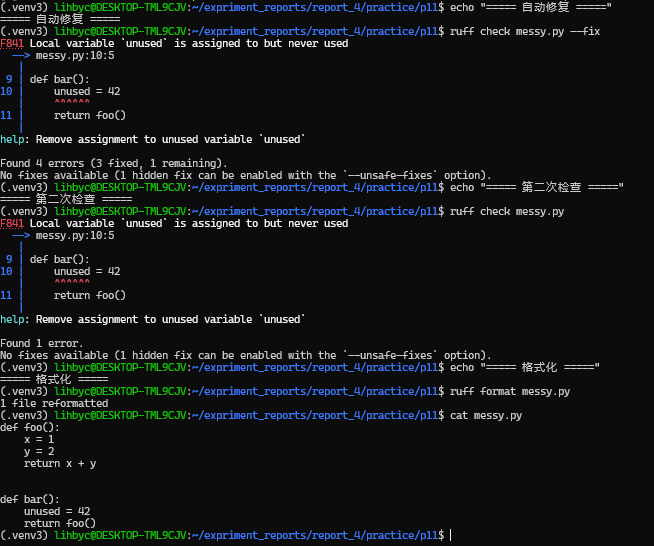
\includegraphics[width=0.85\textwidth]{p113.png}
\textbf{解题感悟}：\texttt{--fix} 只能处理机械问题；未使用变量等涉及语义的，需要人（或 agent）分析后修改。

\vspace{0.3cm}

% ---------- p12 ----------
\subsection*{练习12（p12）：手动补测试提升覆盖率}
\textbf{内容}：从低覆盖率到高覆盖率。

\textbf{操作步骤}：
\begin{enumerate}
    \item 复制 \texttt{calc.py}，先写只覆盖 \texttt{add}/\texttt{sub} 的测试，跑 \texttt{coverage report -m} 得到 60\%。
    \item 补齐 \texttt{mul}、\texttt{div}、\texttt{div\_zero}（异常分支）的测试，覆盖率升至 100\%。
    \item \texttt{coverage html} 生成可视化报告。
\end{enumerate}

\textbf{结果}：
\begin{lstlisting}
Name           Stmts   Miss  Cover   Missing
--------------------------------------------
calc.py           10      0   100%
test_calc.py      13      0   100%
--------------------------------------------
TOTAL             23      0   100%
\end{lstlisting}

\textbf{解题感悟}：异常分支常被忽略，但正是这些分支最容易隐藏缺陷；补齐异常测试对提升覆盖率贡献最大。
\par

\includegraphics[width=0.85\textwidth]{p121.png}
\par

\includegraphics[width=0.85\textwidth]{p122.png}
\vspace{0.5cm}

以上 12 项练习从代码质量、正则、元编程、命令行工具等维度巩固了本周内容，与四道课上检查题形成互补。

\newpage

% ==================== 实验总结 ====================
\section*{实验总结}
\addcontentsline{toc}{section}{实验总结}

通过本周实验，我系统掌握了以下技能：
\begin{itemize}
    \item 本地质量门禁的搭建：\texttt{pyproject.toml} 配置 ruff 与 pytest，\texttt{check.sh} 串联格式检查、静态检查与测试，返回 0 即通过。
    \item Make 依赖图的编写：准确声明数据文件、脚本与中间产物的依赖，实现增量构建与 \texttt{clean} 撤销。
    \item 命令行工具的组合：\texttt{curl} + \texttt{jq} + Markdown 生成可读报告，\texttt{column} / \texttt{@tsv} 输出对齐表格。
    \item 综合交付能力：从修复 bug、构建 wheel、计算 SHA-256 到内容聚焦的 Git 提交，形成完整闭环。
\end{itemize}

同时，我也积累了若干环境与工具使用经验：
\begin{itemize}
    \item 跨目录复制项目时不要连带复制 \texttt{.venv}，应重建虚拟环境。
    \item \texttt{cp -r src dst} 在 \texttt{dst} 已存在时会产生嵌套目录。
    \item \texttt{python -m 模块} 需要模块末尾有 \texttt{if \_\_name\_\_ == "\_\_main\_\_"} 入口才会执行 \texttt{main()}。
    \item \texttt{ruff --fix} 与 \texttt{ruff format} 可能交替修改文件，pre-commit 场景下需要重复 \texttt{add + commit}。
\end{itemize}

\newpage

% ==================== Git 仓库 ====================
\section*{Git 仓库与版本管理}
\addcontentsline{toc}{section}{Git 仓库与版本管理}

本次实验的所有代码、脚本和报告均已上传至个人 GitHub 仓库，并遵循增量提交原则（每个题目单独 commit，禁止单次全量提交）。

\subsection*{仓库地址}
\begin{center}
    \url{https://github.com/lhbyc0718/system_tool_learning}
\end{center}

\subsection*{提交记录}
\begin{itemize}
    \item 每次实验完成后均进行增量提交，每个题目单独 commit。
    \item 提交信息清晰描述改动内容（如“完成第13题：本地质量门禁”、“完成第14题：Makefile 依赖重建”）。
    \item 报告、代码、脚本分类存放，目录结构规范。
\end{itemize}

\subsection*{commit 记录截图}
\begin{figure}[H]
    \centering
    \includegraphics[width=0.9\textwidth]{git_commits_week4_p.png}
    \caption{GitHub 仓库 commit 记录（第四周）}
    \label{fig:git_commits_week4}
\end{figure}

\end{document}
